\documentclass{article}
\usepackage[utf8x]{inputenc}
\usepackage[russianb]{babel}
\usepackage[usenames]{color}
\usepackage{vmargin}
\usepackage{ amssymb }
\usepackage{listings}
\usepackage[linesnumbered,boxed]{algorithm2e}
\usepackage{graphicx}
\usepackage{amsthm}
\usepackage{setspace}
\usepackage{indentfirst}
\usepackage[noend]{algorithmic}
\onehalfspacing
\setpapersize{A4}
\setmarginsrb{3cm}{2cm}{3cm}{2cm}{0pt}{0mm}{0pt}{13mm}
\sloppy
\renewcommand\contentsname{Оглавление}
\renewcommand{\labelenumi}{\theenumi)}

\begin{document}

\null\hfill\begin{tabular}[t]{l@{}}
	\textit{Kirill Zuev}
\end{tabular}

\begin{center}
	\textbf{Home assignment № 4}
\end{center}

\textbf{Task 1.}

\begin{figure}[h!]
	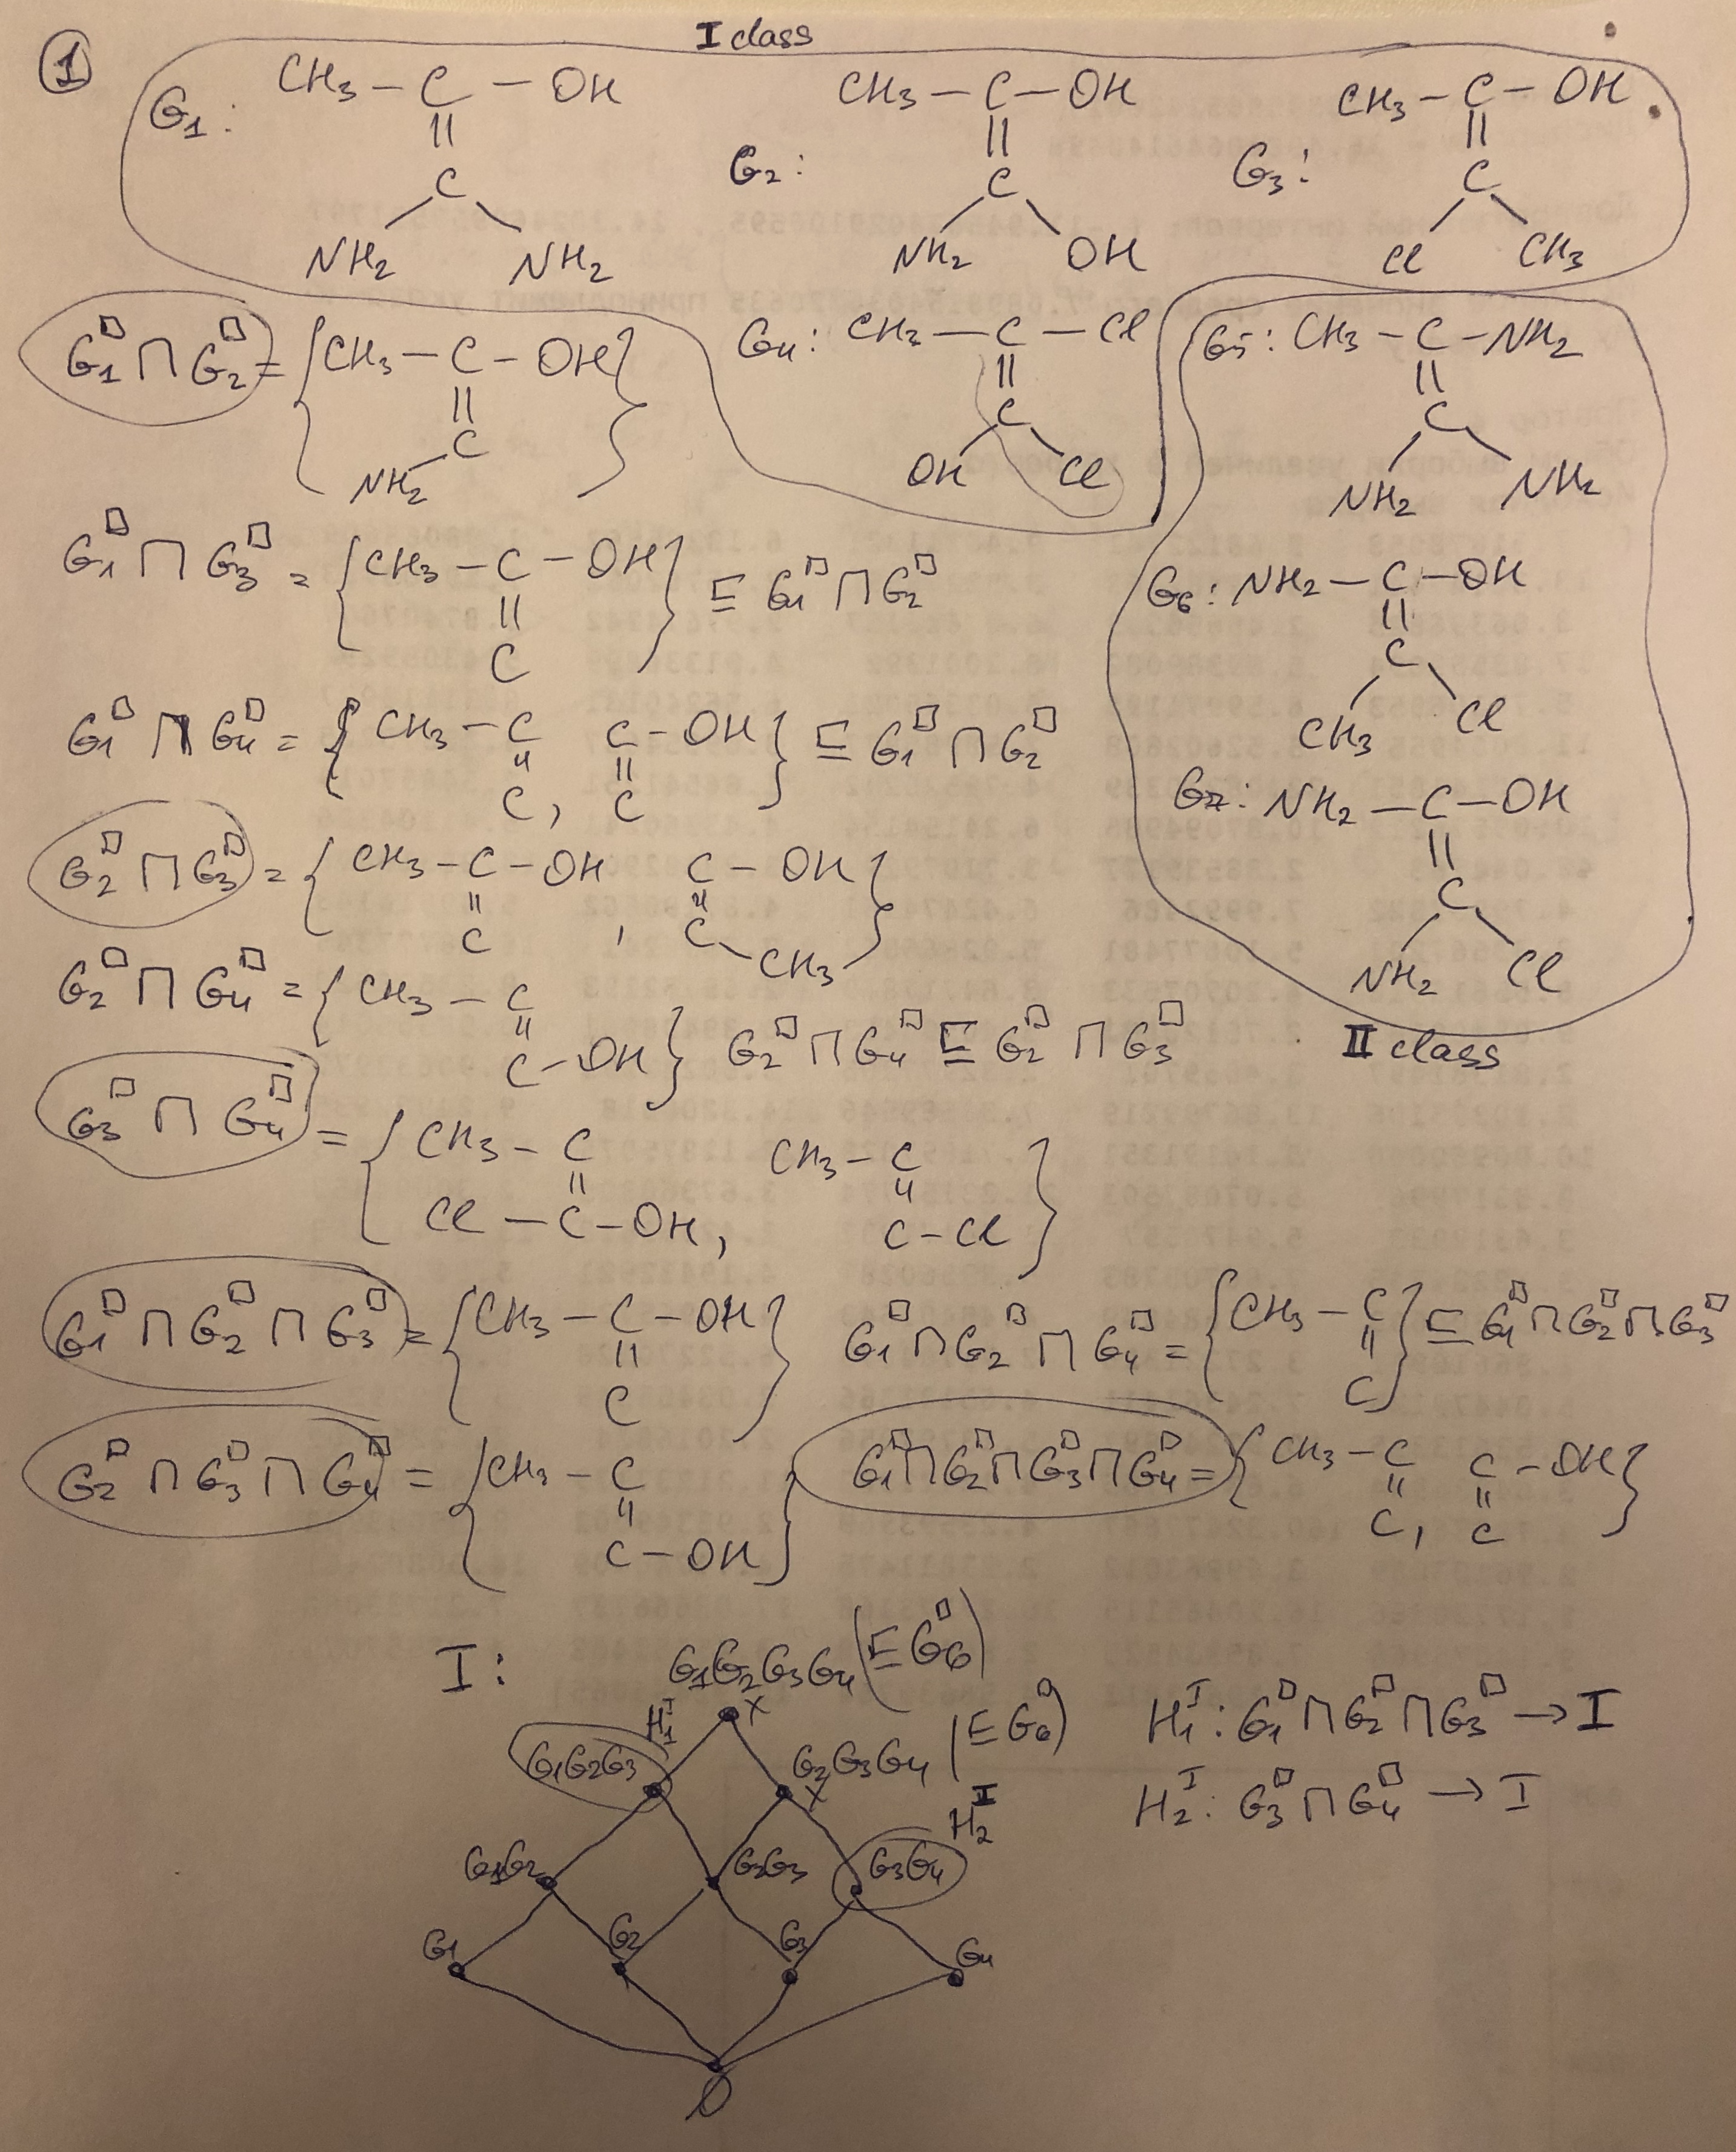
\includegraphics[width=15cm]{1-1.jpg}
\end{figure}
\begin{figure}[h!]
	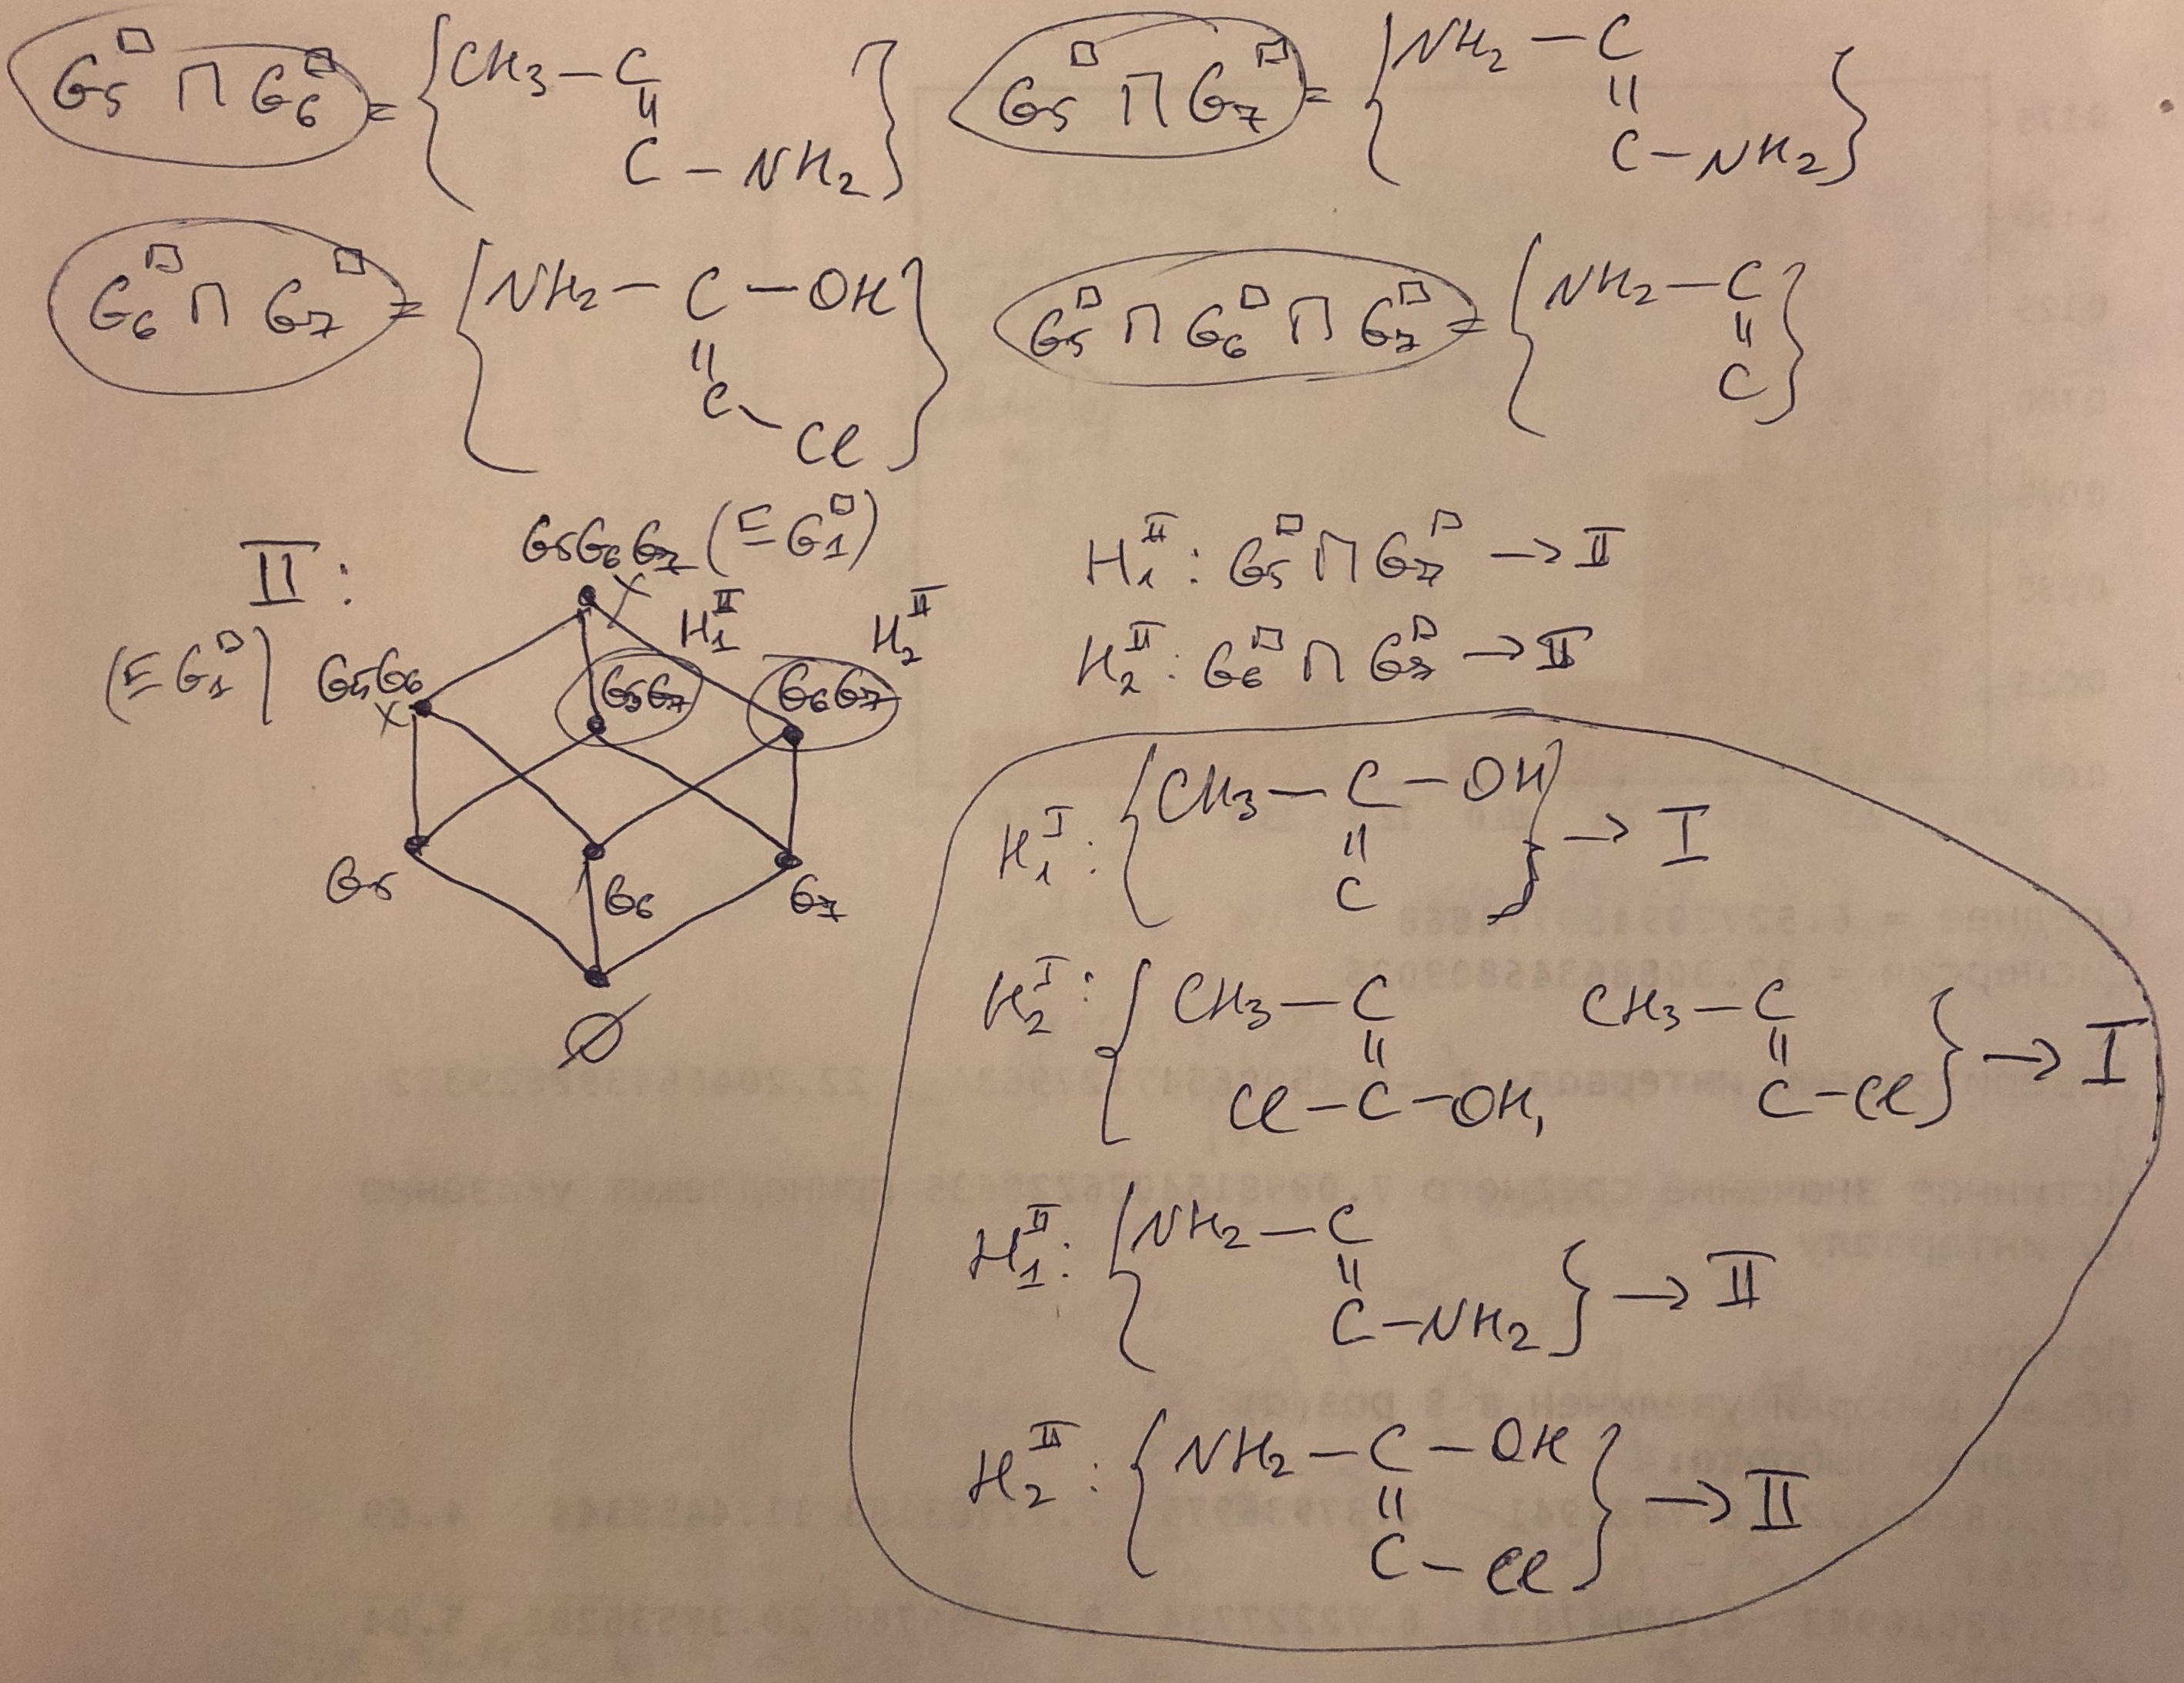
\includegraphics[width=15cm]{1-2.jpg}
\end{figure}
\clearpage

\textbf{Task 2.}

I wrote a Python program (\textit{Task2.ipynb}) including finding all “weak” hypothesis and target classes for test set.\\

\textbf{Task 3.}

I wrote a Python program (\textit{Task3.ipynb}) including lazy classification and a classification rule such that, test objects 1) and 3) will be classified as class 1, and object 2) as class 2.\\

\textbf{Task 4.}

\begin{figure}[h!]
	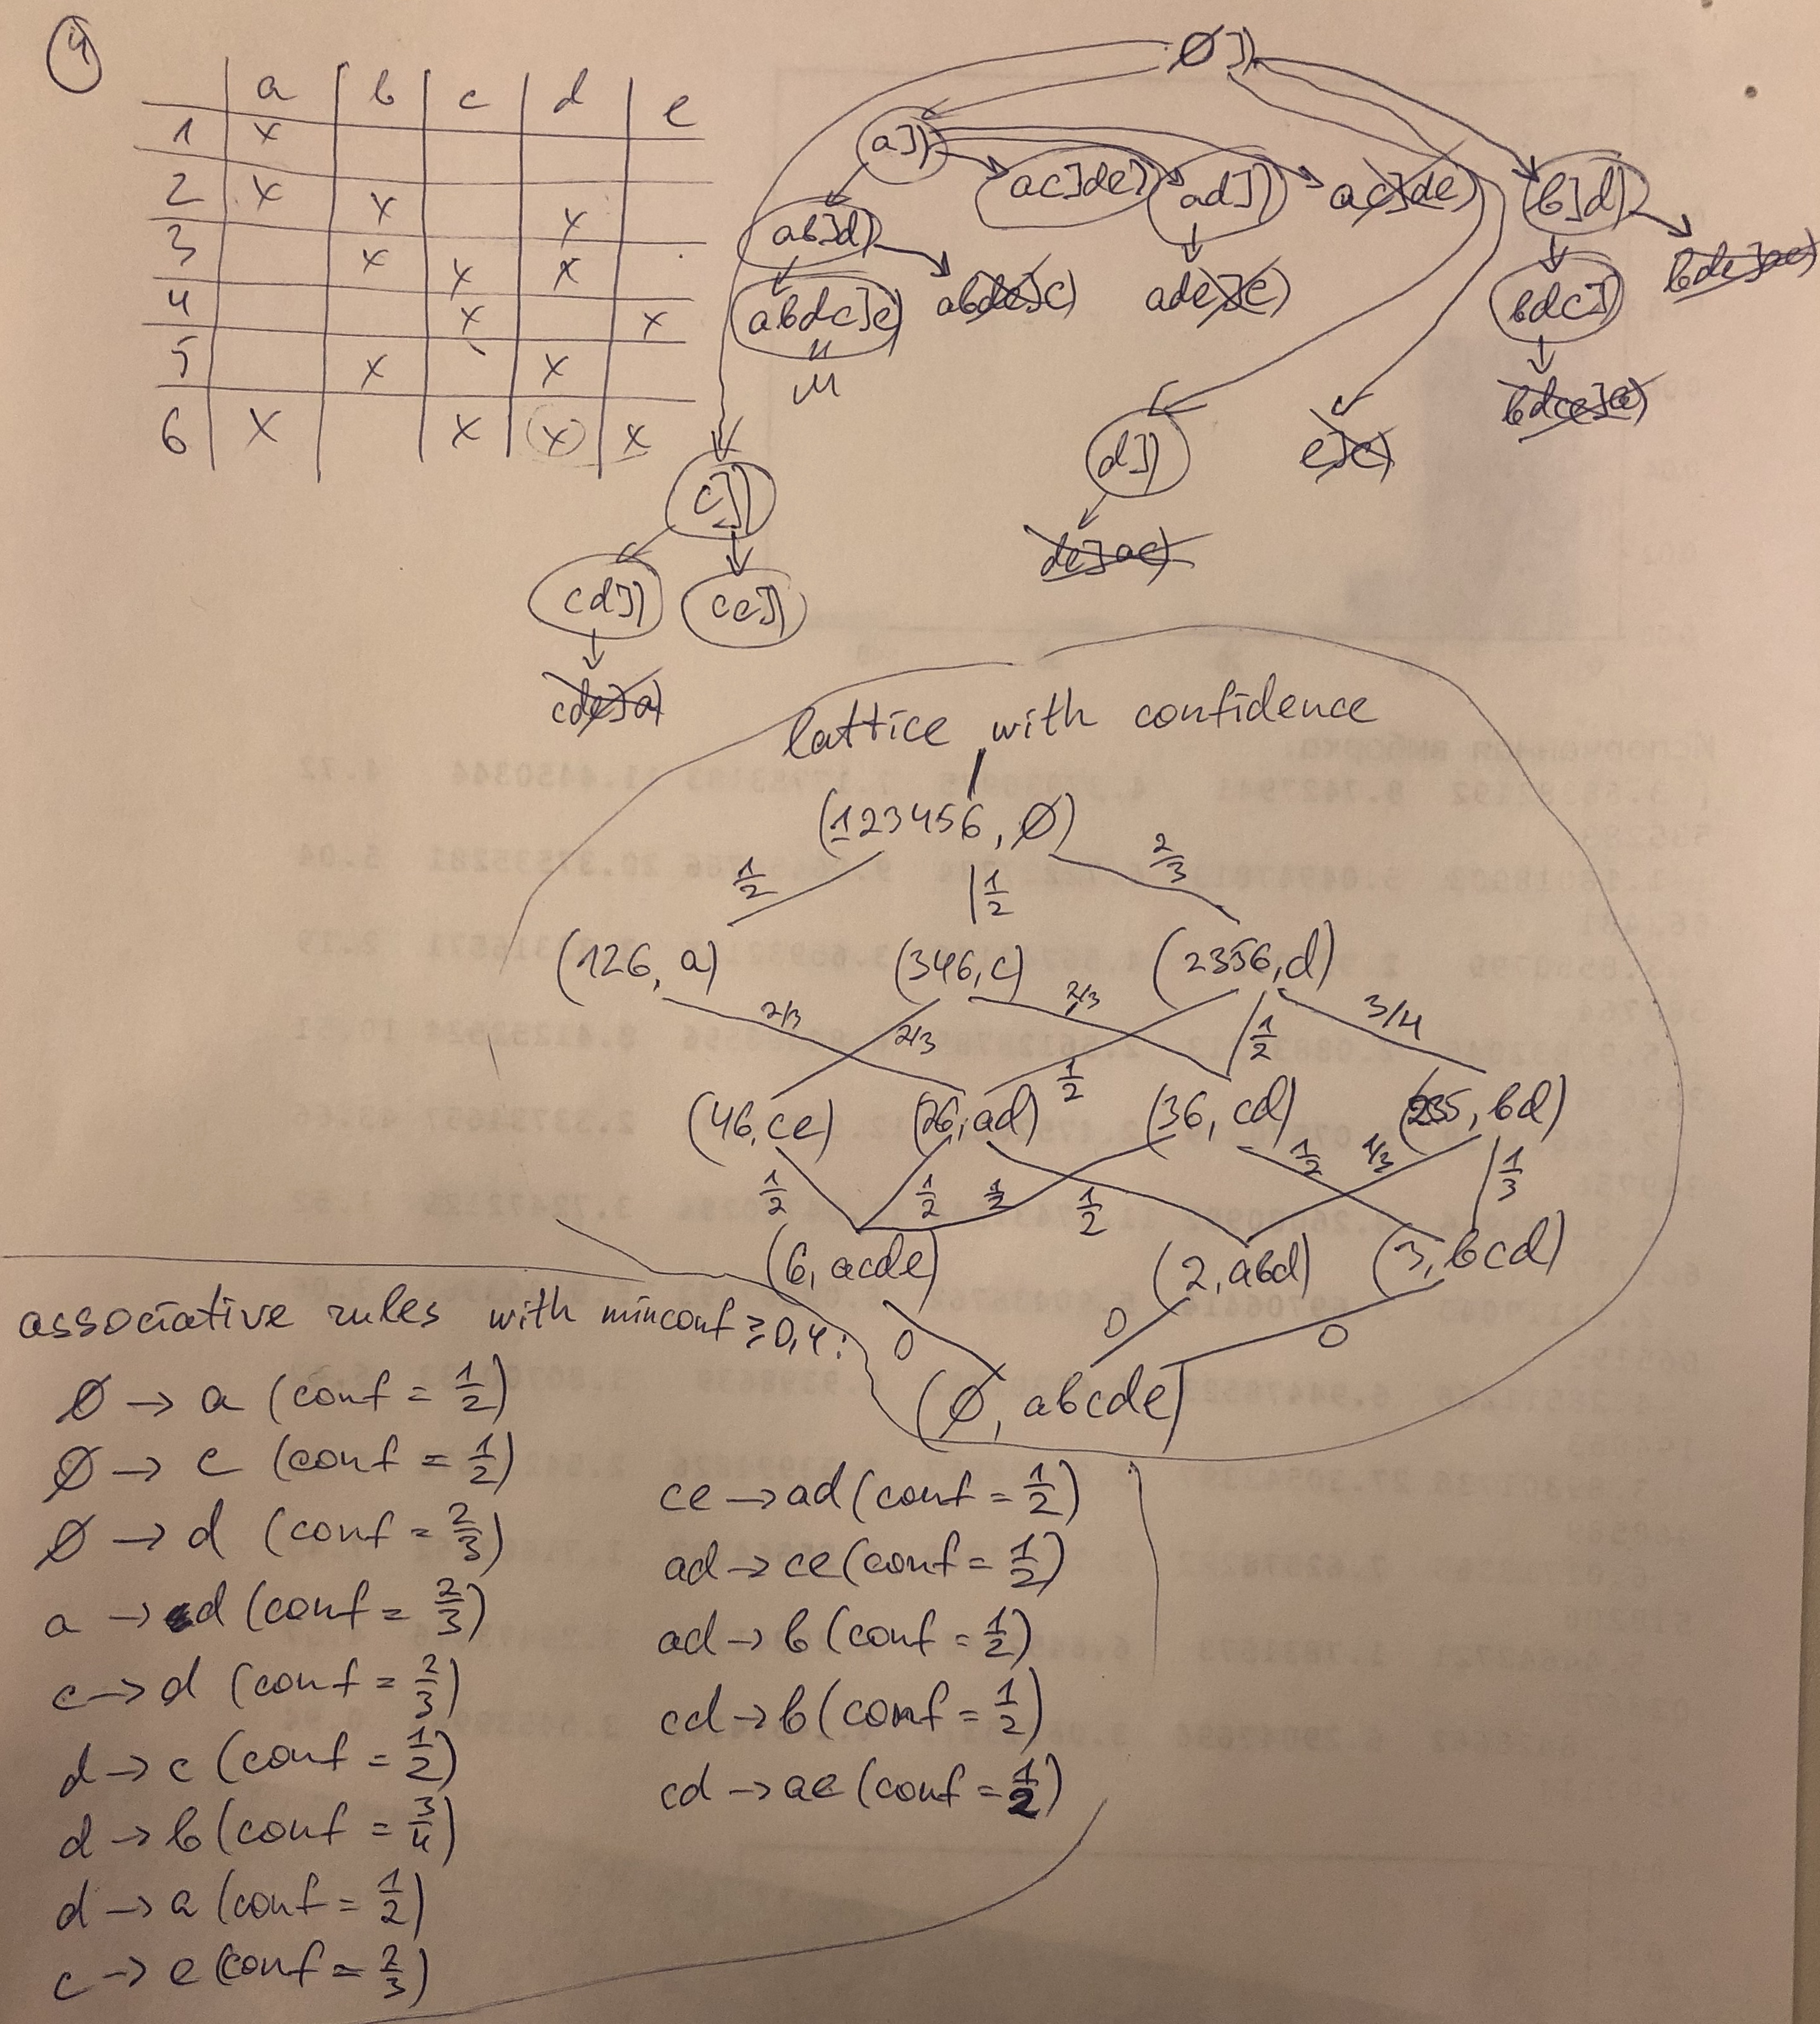
\includegraphics[width=15cm]{4.jpg}
\end{figure}

 \end{document}